\section{Introduction}

% Given the intrinsic complexity when analysing services in distributed
% environments, one normally use different abstractions to describe and
% analyse services. One of such abstractions deals with the the study of
% the concurrent nature of services. Process calculi are formal
% languages conceived for the description and analysis of concurrent
% systems. As such, the goal of a process calculus is to provide a
% rigorous framework where complex systems can be accurately analysed,
% including reasoning techniques (e.g.: type systems, specification logics) to
% verify  essential properties about their behaviour. 
The study of interactions between distributed environments is central
in concurrency theory, and it is the central idea when describing
service oriented architectures. In a service oriented architecture,
the main goal lies in describing the coordination methods so different
participants can distribute and communicate their workloads in such a
way that all those participants can achieve their business goals after
their engagement in a protocol.
The term structured
communications \cite{honda1998lpa} refers to the branch of process
calculi devoted to the analysis of interactions between services. In a
calculus for structured communications, one considers the computation
within a service as an atomic activity, and the focus is on the core
of  the interactions between services. On the technological
side, the use of structured communications is ideal for the study of
service oriented architectures: it allows us to focus only on the
sequences of messages exchanged between participants, and abstracts away details about the local
implementation of services.

Despite their recent appearance, the development of services technologies have
grown constantly, and different but interrelated views
have been proposed. We
can here identify two dichotomies: that of global and local views of
services and that of imperative and declarative specifications. In the first
dichotomy, either one describes the system as the exchange of messages
between different participants, or one considers the system as the
composition of the local behaviours of each participant. In this first
view, known as \emph{choreography} \cite{kavantzas2004web}, one
considers the system as a whole, taking care only of the interfaces
that participants use when interacting to the outside world. In the
second view, known as \emph{orchestration}
\cite{MisraCook06JSSM}, one models the system as seen
by the eyes of each participant (so-called end-point), sending and
receiving messages but not knowing which other actors are present in a
communication. As recently presented
\cite{carbone7scc,DBLP:conf/coordination/BusiGGLZ06,Hongli2007Exploring-the-C}, choreographies and
orchestrations have close ties to each other, and one can 
project a choreography to generate distributed orchestrations that
implements it, sometimes referred to as an \emph{end-point projection}.

The second dichotomy referred to here considers to the approach used to
construct the models. Descriptions can have imperative or declarative
flavours: In an imperative approach, one explicitly defines the control
flow of commands. Typical representatives of this approach are based
on process calculi, and come with behavioural equivalences and type
disciplines as their main analytic tools
\cite{Puhlmann2005Using-the-Pi-Ca,lapadula7cows,boreale2006ssc,honda1998lpa,vieira2008conversation}.
On the contrary, in a declarative approach the focus drifts to the
specification of the set of constraints (causality relations, time
constraints, quality of service) processes should fulfil in order to
be considered correct
\cite{pesic2006daf,vanderaalst2006dtt,DDBP08,NORGAARD2005Method-for-gene}.
Even if these two trends address similar concerns, we find that they
have evolved rather independently from each other. 
% Returning to our
% example, 
% We might consider the specifications above presented
% imperative specifications, whereas a declarative specification will
% let parts of the process unspecified. 
% For instance, we could relax the
% specification given above by accepting any implementation of AC that
% complies with an ordering of actions where it first receives the
% booking data, and eventually (that is, immediately or in an
% unspecified sequence of interactions) returns a booking offer. Such a
% policy can be observed better on a logical formalisation, as for
% instance a formula in Linear Temporal Logic \cite{manna1992temporal}.

This chapter presents for the first time a framework were both the
global and local visions, and declarative and imperative
specifications can live together. The approach starts by providing a
logical characterisation of choreographies, allowing flexible
specifications where not all interactions need to be
specified. Secondly, it provides a logical characterization of
orchestrations, to allow descriptions of their local points of view in
a declarative manner. Third, it provides the connections between
global and local formulae, so one can project properties described at
the level of choreographies to the parallel composition of formulae at
the level of endpoints. Finally, the framework is endowed with 
verification techniques in the form of proof systems, that allow one
to verify whether a specification satisfies a formulae both at
the level of choreographies and at the level of orchestrations.


A framework combining both declarative and imperative aspects in
structured communications can be useful in a practical setting. In
software development, the two classical languages for
describing interactions are WS-CDL \cite{kavantzas2004web} (for choreographical
specifications) and WS-SDL \cite{christensen2001web} (for orchestrations). In WS-CDL, one
describes a service oriented application with knowledge of all
participants that will be included in the protocol. Every time one
needs to change a parameter (e.g.: the name of the participants, or
the names of the variables in the exchanged messages) the scenario has
to be regenerated, and their endpoints tested for compliance again. A
more complicated scenario involves the inclusion of \emph{new
  activities} in the model. It is highly probable that the existing
battery of tests generated for the choreography will serve of no use
here, as the sequence of interactions have been broken. With tests
defined in terms of logical formulae, one impose an ordering only on those
sequences of activities that must occur, leaving all the other
scenarios open. Sequences of interactions can also be more flexible,
as they might consider that a given sequence will eventually achieve
its satisfactory state. With this extra level of flexibility,
different versions of the same choreography featuring few or more
details can be proven equally satisfactory, as far as they satisfy the
same logical property. 

A similar scenario occurs in the realm of
orchestrations. In WS-SDL, the testing of an end-point involves two
phases: the testing of its internal logic, and the testing of the
interactions between the end-point and the environment. Having a
complete picture of all services  in an environment is a
rather hard task, as each end-point can make service calls to end-points
located inside their internal domain, complicating a verification task
based on a global knowledge. A declarative approach aims at mitigating
this problem, as end-point properties will be satisfied only when the
necessary services are present, and the correct flows between
interactions are respected.



\subsection{An Example}

The notions of the framework are easily explained through an example
describing each of the different visions we integrate. 

Let us consider an electronic booking scenario.  On one side, consider
a company AC which offers flights directly from its website. On the
other side, there is a customer looking for the best offers.  In this
scenario, the customer establishes a communication with AC and asks
for a flight proposal given a set of constraints, such as the
destination, the dates allowed, etc. After receiving a request and
checking its validity, AC establishes a communication with its partner
AC' serving the destination asked by the customer, and forwards the
request made by the customer to AC'. Once that AC' is able to process
the request, he can contact the customer and provide him an offer. The
ways AC' communicates the offer to  the customer are \emph{purposely} left unspecified:
for instance, 1) AC' could reply back to AC, that he would later contact
the customer with their previous established session, or 2) AC' receives from AC the session key of the
communication established between the customer and AC, and uses it to
reply back to the customer (\emph{delegation})\footnote{This option,
  although interesting, will be refrained from consideration in our
  current study, as the choreography language utilised does not
  feature delegation of sessions}, or 3) AC' could
create a new session with the customer, and send him the offer
directly. A graphical specification of the
interaction diagrams corresponding to such cases is illustrated  in Figure
\ref{Logic4Struct:introduction::example}.


\begin{myfigure}{t} \vspace{1cm}
     \centering
     \begin{subfigure}[b]{0.65\textwidth}
       \centering
       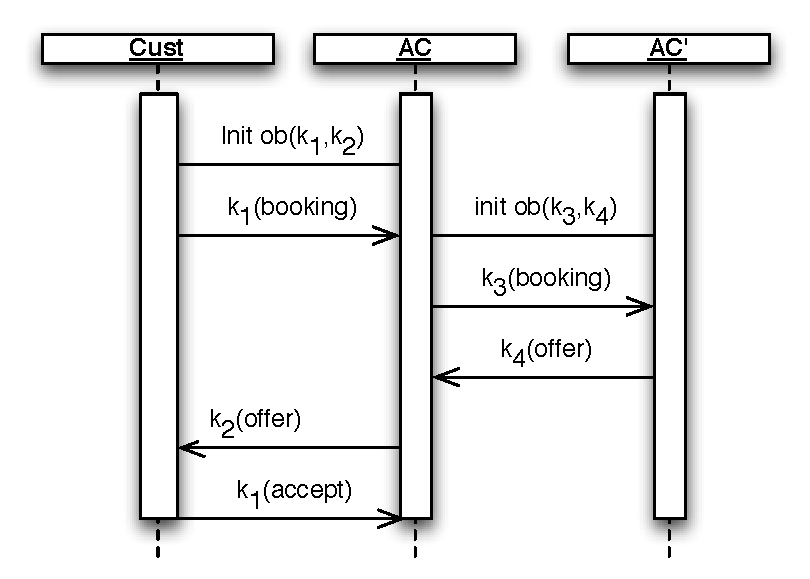
\includegraphics[width=1.00\textwidth]{LogicalProjection-introExample-welltyped}
       \caption{Interaction diagram (following classical session types)}
     \end{subfigure} \\
     \begin{subfigure}[b]{0.65\textwidth}
       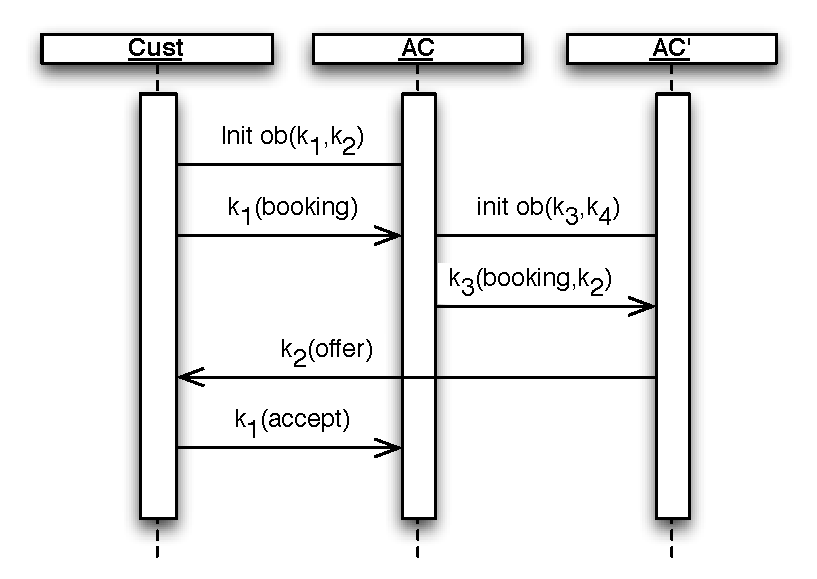
\includegraphics[width=1.00\textwidth]{LogicalProjection-introExample-delegation}
       \caption{Interaction diagram (session types with delegation)}
       \centering
     \end{subfigure} 
    \caption{Electronic booking example}
    \label{Logic4Struct:introduction::example}
\end{myfigure}



  A global specification focuses on the description of the
  interactions between participants $Cust, AC$ and $AC'$. For
  instance, $\init{\text{Cust}}{\text{AC}}{\text{ob}_{AC}}{k_1} $
  initiates an interaction between the Customer and the service
  $ob_{AC}$ located in the Airline company, labelled with a session
  identifier $k_1$. Similarly, the communication of the offer message
  between the Airline partner and the customer will be written as
  $\interact{\text{AC'}}{\text{Cust}}{k_2}{\text{offer}}{y}
  $. Choreographies $C_{OB-i}$ present possible specifications of 
  message exchanges in Figure
  \ref{Logic4Struct:introduction::example}, where  $C_{OB-1}$
  presents the alternative where messages travel back through AC,
  $C_{OB-2}$ the alternative creating a new session, and $C_{OB-3}$
  the alternative using session delegation.
  Notice that, in order for models like the ones described in $C_{OB-2}$
  and $C_{OB-3}$ to respect the causality and coherence relations
  between interactions present in the theory of
  session types, we need languages to
  be expressive enough to support further capabilities, like delegation \cite{honda1998lpa} and correlation sets
  \cite{lapadula7cows}. 

  \begin{align} \label{Logic4Struct:intro::example}
  C_{OB-1} = {} & \init{\text{Cust}}{\text{AC}}{\text{ob}_{AC}}{k_1,k_2} \pfx
  \interact{\text{Cust}}{\text{AC}}{k_1}{\text{booking}}{x_1} \pfx
  \notag \\
  & \init{\text{AC}}{\text{AC'}}{\text{ob}_{AC'}}{k_3,k_4} \pfx
  \interact{\text{AC}}{\text{AC'}}{k_3}{x_1}{y}  \pfx  \notag\\
  & \interact{\text{AC'}}{\text{AC}}{k_4}{\text{offer}}{x_2} \pfx
   \interact{\text{AC}}{\text{Cust}}{k_2}{x_2}{c}  \pfx \notag\\
   & \interact{\text{Cust}}{\text{AC}}{k_1}{\text{accept}}{z}
%    \\[0.5cm]
\end{align}
\begin{align}
  C_{OB-2} = {} & \init{\text{Cust}}{\text{AC}}{\text{ob}_{AC}}{k_1,k_2} \pfx
  \interact{\text{Cust}}{\text{AC}}{k_1}{\text{booking}}{x} \pfx
  \notag \\
  & \init{\text{AC}}{\text{AC'}}{\text{ob}_{AC'}}{k_3} \pfx
  \interact{\text{AC}}{\text{AC'}}{k_3}{k_2}{x'}  \pfx  \notag\\
  & \interact{\text{AC'}}{\text{Cust}}{k_2}{\text{offer}}{y} \pfx
  \interact{\text{Cust}}{\text{AC}}{k_1}{\text{accept}}{z} 
% \\[0.5cm]
\end{align}
\begin{align}
  C_{OB-3} = {} & \init{\text{Cust}}{\text{AC}}{\text{ob}_{AC}}{k_1,k_2} \pfx
  \interact{\text{Cust}}{\text{AC}}{k_1}{\text{booking}}{x_1} \pfx
  \notag \\
  & \init{\text{AC}}{\text{AC'}}{\text{ob}_{AC'}}{k_3,k_4} \pfx
  \interact{\text{AC}}{\text{AC'}}{k_3}{x_1}{y}  \pfx  \notag\\
  & \init{\text{AC'}}{\text{Cust}}{\text{ob}_{Cust}}{k_5,k_6} \pfx
  \interact{\text{AC'}}{\text{Cust}}{k_5}{\text{offer}}{c} \pfx \notag\\
  & \interact{\text{Cust}}{\text{AC}}{k_1}{\text{accept}}{z}
  \end{align}




  In the same way that a choreographical specification describes each
  of the interactions between participants, a logical characterisation
  of choreographies denotes formulae describing the evolution of such
  interactions. However, a logical characterisation gives more
  flexibility to the specification of interactions: One can forget
  about the addition of extraneous constructs of the language and
  define a simple policy about the behaviour of interactions. This
  policy can be described using logical
  specification over choreographies.  This logical
  specification describes \emph{only} the important parts of the message flow
  between participants. For instance, in the above presented
  specification, one can describe a property ensuring that, given a
  communication between the Customer and the Airline company with a
  booking message, there is an eventual response directed to the
  customer with an offer matching the same session identifier (in
  this case, not necessarily coming from the same participant the
  communication was initiated).

  {
    \begin{align} \label{Logic4Struct:intro::globalProperty}
      C_{OB-i} |= & \exists A,k_r  \pfx
      \actionF{\initF{Cust}{AC}{ob_{AC}(k_1,k_2)}} \pfx \actionF{\comF{Cust}{AC}{k_1
          (\text{booking}) }} \pfx \notag \\ 
      & \may \actionF{\comF{A}{Cust}{k_r (\text{offer}) }} 
    \end{align}
  }

  In a similar but orthogonal approach, the same specification in
  equation \ref{Logic4Struct:intro::example} can be seen as processes
  implementing each participant involved in the choreography. For
  instance, an interaction $\chor =
  \init{\text{Cust}}{\text{AC}}{\text{ob}_{AC}}{k_1,k_2} \pfx \chor'$
  describing session initiation can be decomposed to concurrent
  processes $\chor_{\text{Cust}} \pp \chor_{\text{AC}}$ implementing
  each side of the interaction:

  \begin{displaymath}
    \xymatrix{ 
      & \init{\text{Cust}}{\text{AC}}{\text{ob}_{AC}}{k_1,k_2} \pfx \chor'
      \ar@{->}[dr]^{\mathcal{\chor_{\text{AC}}}} \ar[dl]_{ \chor_{\text{Cust}}} &  \\ 
      \initOut{ob_{AC}}{k_1,k_2} \pfx \chor'_{\text{Cust}}  & \pp & \repInitIn{ob_{AC}}{k_1,k_2} \pfx \chor'_{\text{AC}}} 
\end{displaymath}

The full set of projections realising the choreography in equation
\ref{Logic4Struct:intro::example} might need to include participants Cust, AC and
AC', and will need to guarantee that the ordering of the messages
imposed in the global specification is still reflected in the
projections. The resulting behaviour can be seen below:

\begin{align} 
  \chor_{\text{Cust}} = {} & \initOut{ob_{AC}}{k_1,k_2} \pfx
  \send{k_1}{\text{booking}} \receive{k_2}{c}
  \send{k_1}{\text{accept}} \INACT \label{Logic4Struct:intro::endPoint::customer}\\
  \chor_{\text{AC}} ={} & \repInitIn{ob_{AC}}{k_1,k_2} \pfx \receive{k_1}{x_1}
  \initOut{ob_{AC'}}{k_3,k_4} \pfx \send{k_3}{x_1} \receive{k_4}{x_2}
  \send{k_2}{x_2} \receive{k_1}{z}\INACT \\
  \chor_{\text{AC'}} ={} & \repInitIn{ob_{AC'}}{k_3,k_4} \pfx\receive{k_3}{y}
  \send{k_4}{\text{offer}} \INACT \\
  \chor = {} & \chor_{\text{Cust}} \pp \chor_{\text{AC}} \pp \chor_{\text{AC'}}  \label{Logic4Struct:intro::endPoints}
\end{align}

A declarative vision of end points allows us to express properties
regarding each of the participants involved. For instance, we can
check that the end point representing the customer
respects a property stating that there is an eventual reply back after
having made a booking request. 
 Hence, the end point specification at Equation
\ref{Logic4Struct:intro::endPoint::customer} needs to satisfy the following formula:


\begin{align}
   \chor_{\text{Cust}} |=&
   \locatedActionF{Cust}{\asynchOutputF{k_1}{\text{booking}}} \pfx
   \may ~   \locatedActionF{Cust}{\asynchInputF{k_2}{x}} \pfx \endF
\end{align}

In the above,  $\locatedActionF{Cust}{\psi}$ denotes the execution of an action
$\psi$ by participant $Cust$.

An interesting point here is the relation we can evidence
between declarative specifications at global and local
viewpoints. In principle, a declarative model describing the behaviour
at the level of choreographies needs to be projected to formulae
describing the behaviour of their end-points.  Let $\phi_{OB}$ the formula
in Equation \ref{Logic4Struct:intro::globalProperty}, and its
decomposition into end-point formula described below:


\begin{align}
  [| \phi_{OB} |] = & \exists A, k_r. 
  (\locatedActionF{Cust}{\asynchServiceOutF{ob_{AC}}{k_1,k_2}} \pfx
  \locatedActionF{Cust}{\asynchOutputF{k_{1}}{\text{booking}}}  \\
   & \qquad \pfx ( \locatedActionF{Cust}{\asynchInputF{k_{r}}{\text{offer}}} \lor
   \may \locatedActionF{Cust}{\asynchInputF{k_{r}}{\text{offer}}} )) \notag
   \\
   & \pp (\locatedActionF{AC}{\asynchServiceInputF{ob_{AC}}{k_1,k_2}}
   \pfx   \locatedActionF{AC}{\asynchInputF{k_{1}}{\text{booking}}})
   \notag\\
   & \pp (\locatedActionF{A}{\asynchInputF{k_{r}}{\text{offer}}} \lor
   \may \locatedActionF{A}{\asynchInputF{k_{r}}{\text{offer}}})
\end{align}

The formula projected \emph{only} speaks about the projected behaviour
from the global specification, and allows for multiple implementations
of services to satisfy this specification. We will see later, that
although the translation seems intuitive, it is far from trivial: end
points can implement many threads at the same time, and those have to
be included in consideration on translations of the logical
formulae. Also, the projections considered should be
\emph{meaningful}, in the sense that they respect the theory of end
point projections. We show in further sections how this is accomplished.


\paragraph{Contributions}
Here we present a framework integrating imperative and declarative
views for structured communications. Building from previous research
in calculi for the specification of services, we
provide modal logic characterisations of the interactions occurring in
a system, both from a global point of view and from the point of view
of individual participants. The framework cope with two aims: exhibiting logical
guarantees about the presence of an interaction, and model generation
from logical specifications. In particular, we present two logical
languages for describing choreographies and orchestrations. First, \GL
is a logic describing possible interactions in a choreographical
language (the global calculus): the correspondence between
specifications in the calculus and the logic is tight, and one can go
either from the logical characterisation to the process algebraic
specification of a process, or prove that a choreographical
description respects a formula in \GL\!\!. Second, \LL is a logic
inspired by Hennessy-Milner with the aim of describing properties
about the interactions in a language of orchestrations (the end-point
calculus). The logic characterises typed bisimulation (pruning). As
the main result, we show that there is a correspondence between
imperative and declarative descriptions of the projections from
choreographies to its end-points. 


We pay special attention to the correspondence between imperative and
declarative descriptions for structured communications. The
correspondence presented here relies on the existence of meaningful
projections of choreographies to their corresponding end-points.  The
mapping is far from trivial, and needs to preserve causal relations
between messages and threads, namely connectedness, well-threadedness
and coherence. The theory describing mappings of this kind is normally
referred to as end-point-projections \cite{carbone7scc}, and is
achieved by equipping the global and the end-point calculus with
behavioural types.  Our main result in Theorem
\ref{Logic4Struct:theorem:lp:soundness} implies that for a well-typed
choreography $\chor$, and an associated choreographical formula
$\phi$, then 1) $\chor$ has a meaningful projection to end-point
behaviour, 2) $\phi$ has a logical projection to meaningful end-point
formulae, and 3) That satisfaction at the level of choreographies and
at the level of end-points coincide. This result relies on the use of
the type systems in \cite{carbone7scc}, which are included here for
completeness. A reader familiar with such type systems can easily skip
Section \ref{Logic4Struct-GlobalTypes},
Section\ref{Logic4Struct-EndPointTypes} and Section
\ref{Logic4Struct:sec:epp-types}.




\subsubsection{Overview of the document}

In Section \ref{Logic4Struct:sec:globalCalc} we give a summary of the
formal foundations of a calculus of choreographies, the so-called
global calculus. Its respective logic is presented in Section
\ref{Logic4Struct:sec:globalLogic}. We present undecidability results
for the logic on the global calculus in Section
\ref{Logic4Struct:sec:undecidability}. A proof
system relating the logical characterisation and the recursion-free
fragment of the global calculus shown in Section
\ref{Logic4Struct:sec:proofSys}. The semantics for the calculus of
end-points is presented in Section \ref{Logic4Struct:sec:epc}, a
logical characterisation of the end-point calculus is presented in
Section \ref{Logic4Struct:sec:localLogic}, as well as the main
contribution of this paper, namely the correspondence between the
end-point projection and the logical projection between global and
local formulae. Finally, concluding remarks are presented in Section
\ref{Logic4Struct:sec:conclusion}.


% When analysing service oriented systems, either we describe the system
% as the exchange of messages between different participants, or we
% consider the system as the composition of the local behaviours of each
% participant.  In this first view, known as \emph{choreography}, we
% consider the system as a whole, taking care only of the interfaces
% that participants use when interacting to the outside world. In the
% second view, known as \emph{orchestration}, we model the system as
% perceived by the eyes of each participant, sending and receiving
% messages but not knowing which other actors are present in a
% communication. A good illustration can be seen in the way a soccer
% match is planned: the coach has an overall view of the team, and
% organise how players will interact in each play (the role of a
% choreography) while each player performs his role by interacting with
% each of the members of his team by throwing/receiving passes. The way
% each player synchronise with other members of the team represents the
% role of an orchestration.
 
 
% The link between choreography and orchestration has been proposed in
% \cite{carbone7scc}. Here, choreography and orchestration constitute
% two interrelated approaches for modelling services. Two languages are
% proposed: A Global calculus to model choreographies and the End Point
% calculus to model orchestrations. Additionally, global and local
% specifications has already been shown operational correspondent under
% certain conditions, and one can generate an orchestrated model of a
% choreography by a mapping from the Global calculus to the End Point
% Calculus (something known as the \emph{End Point Projection (EPP)}).


% In this paper we aim at leveraging the trustworthiness level of a
% system by providing a clear methodology of specification and
% verification of structured communications.  Our goal is to provide
% service oriented systems with a \emph{logical characterisation}, both
% from the global perspective and from their end-point
% projections. Figure \ref{Logic4Struct:fig:serviceVerification} illustrates the
% approach for the specification and verification of service-oriented
% systems. We can analyse a choreography $C$ either by mapping a
% specification of global behaviour to a formula $\phi_C$ describing the
% interaction between participants, and from here generate $\bigcap_i [|
% \phi_i |]$, a set of formulas describing the local behaviour of each
% participant. Similarly, we can start from choreography $C$ and then
% use an end point projection to generate the parallel composition of
% the local behaviours of each participant involved in the communication;
% from here we can study their logical meaning as the set of formulas
% generated for each participant, closing the verification square.

% \begin{figure}[t]
% \begin{displaymath} 
% \xymatrix{ 
% C \ar@{<->}[r]^{\mathcal{GL}} \ar[d]_{EPP} &  \phi_C  \ar[d]^{?} \ar[dl]^{?} \\ 
% \prod_i[|P_i|] \ar@{<->}[r]_{\mathcal{LL}}  & \bigcap_{i}[|\phi_i |] } 
% \end{displaymath}
% \caption{Methodology for Service - Oriented Verification}
% \label{Logic4Struct:fig:serviceVerification}
% \end{figure}



% The end point projection between global and local specifications has
% been previously presented in \cite{carbone7scc}, and their operational
% correspondence property allow us to move from local to global
% perspectives and vice versa. Similarly, in a recent work
% \cite{Berger2008Completeness-an} a Hennessy-Milner logic for typed
% \mipi-calculi is introduced, providing the link between local
% specifications and logics.

% In this document we provide the link between choreographies and a
% logics (denoted as $\mathcal{GL}$ in Figure
% \ref{Logic4Struct:fig:serviceVerification}). Starting with an extension of
% Hennesy-Milner logic \cite{hennessy1980observing}, we provide a proof
% system that allows for property verification of choreographies. The
% logic is sound,
% %and complete
% in terms that a choreography will always reflect a logical state of
% the system.
% % , and a logical formula can always represent the state of a
% % choreography. Completeness also allows for checking of partial
% % specifications: if a property describing partial behaviour of the
% % system can be entailed by a choreography, then the whole system
% % would be able to fulfil such a property.
% Furthermore, a final step would conclude a methodology for
% verification of structured communications. The logic for
% choreographies should have a correspondent mapping to a logic to
% reason about end-point projections. \marginpar{fix this part!} This
% step, denoted by the transformation $LP$ between Global and Local
% formulas, is left as as further work of the current document.

% This paper is organised as follows: In section \ref{Logic4Struct:sec:globalCalc} we
% describe the global calculus as our reference language, with its
% syntax and operational semantics. Section \ref{Logic4Struct:sec:globalLogic}
% presents a logical language to express properties about
% choreographies, giving several examples of its use. Section
% \ref{Logic4Struct:sec:proofSys} presents the proof system and correctness results
% while in \ref{Logic4Struct:sec:conclusion} we discuss the future work.
% \marginpar{add part about GL and LL}

%%%%%%%%%%%%%%%%%%%%%%%%%%%%%%%%%%%%%%%%%%%%%%%%
% Introduction used in PLACES 2010                                                 %
%%%%%%%%%%%%%%%%%%%%%%%%%%%%%%%%%%%%%%%%%%%%%%%%

% \section{Introduction}
% Due to the continuous growth of technologies, software development is
% recently shifting its focus on communication, giving rise to various
% research efforts for proposing new methodologies dealing with higher
% levels of complexity. A new software paradigm, known as {\em
%   choreography}, has emerged with the intent to ease programming of
% communication-based protocols. Intuitively, a choreography is a
% description of the global flow of execution of a system where the
% software architect just describes which interactions \emph{might} take
% place. This idea differs from the standard approach where the
% communication primitives are given for each single entity
% separately. A good illustration can be seen in the way a soccer match
% is planned: the coach has an overall view of the team, and organises
% (a priori) how players will interact in each play (the role of a
% choreography); once in the field, each player performs his role by
% interacting with each of the members of his team by throwing/receiving
% passes. The way each player synchronise with other members of the team
% represents the role of an orchestration.
% %  A good illustration can be seen in the way a soccer match
% % is planned: the coach has an overall view of the team, and (a priori)
% % organises how players will interact in each play (the role of a
% % choreography). Instead, at run-time, each player performs his role by
% % interacting with each of the members of his team by throwing/receiving
% % passes according to what the coach has previously described.

 
 
% % The link between choreographies and orchestration has been proposed
% % in \cite{carbone7scc}. Here, choreographies and orchestration
% % constitute two interrelated approaches for modelling services. Two
% % languages are proposed: A Global calculus to model choreographies
% % and the End Point calculus to model orchestrations. Additionally,
% % global and local specifications has already been shown operational
% % correspondent under certain conditions, and one can generate an
% % orchestrated model of a choreography by a mapping from the Global
% % calculus to the End Point Calculus (something known as the \emph{End
% %   Point Projection (EPP)}).


% % In this work we focus on providing service oriented systems with a
% % \emph{logical characterisation} from a global perspective.  We can
% % analyse a choreography either by mapping a specification of global
% % behaviour to a formula describing the interaction between
% % participants.
% % Similarly, we can start from choreography and then use
% % an end point projection to generate the parallel composition of the
% % local behaviours of each participant involved in the communication;
% % from here we can study their logical meaning as the set of formulas
% % generated for each participant, closing the verification square.

% % \begin{figure}[ht]
% %   \begin{displaymath}
% % % \xymatrix{ 
% % % C \ar@{<->}[r]^{\mathcal{GL}} \ar[d]_{EPP} &  \phi_C  \ar[d]^{LP} \\ 
% % % \prod_i[|P_i|] \ar@{<->}[r]_{\mathcal{LL}}  & \bigcup_{i}[|\phi_i |] } 
% % \end{displaymath}
% % \caption{Methodology for Service - Oriented Verification}
% % \label{Logic4Struct:fig:serviceVerification}
% % \end{figure}



% % The end point projection between global and local specifications has
% % been previously presented in \cite{carbone7scc}, and their
% % operational correspondence property allow us to move from local to
% % global perspectives and vice versa. Similarly, in a recent work
% % \cite{Berger2008Completeness-an} a Hennessy-Milner logic for typed
% % \mipi-calculi is introduced, providing the link between local
% % specifications and logics.

% The work in \cite{CHY:dcm2006} formalises the notion of choreography
% in terms of a calculus, dubbed the {\em global calculus}, which
% pinpoints the basic features of the choreography paradigm. Although
% choreography provides a good abstraction of the system being designed
% allowing to {\em forget} about common problems that can arise when
% programming communication e.g. races over a channel, it can still have
% complex structures hence being often error prone. Additionally,
% choreography can be non-flexible in early design stages where the
% architect might be interested in designing only parts of a system as
% well as specifying only parts of a protocol (e.g. initial and final
% interactions). In this view, we believe that a logical approach can
% allow for more modularity in designing systems e.g. providing partial
% specification of a system using the choreography paradigm.

% In this document, we attempt to provide a link between choreography
% and logics. Starting with an extension of Hennessy-Milner logic
% \cite{hennessy1980observing}, we provide the syntax and the semantics
% of a logic for the global calculus as well as several examples
% pointing out the usefulness of the method. Moreover, we provide a
% proof system that allows for property verification of choreographies
% and show that it is
% sound. % Furthermore, a final step would conclude a
% % methodology for verification of structured communications. The logic
% % for choreographies should have a correspondent mapping to a logic to
% % reason about end-point projections. This step, denoted by the
% % transformation $LP$ between Global and Local formulas, is left as as
% % further work of the current document.
 
%%% Local Variables: 
%%% mode: latex
%%% TeX-master: "../Thesis"
%%% End: 
